% Options for packages loaded elsewhere
\PassOptionsToPackage{unicode}{hyperref}
\PassOptionsToPackage{hyphens}{url}
%
\documentclass[
  11pt,
]{article}
\usepackage{amsmath,amssymb}
\usepackage{iftex}
\ifPDFTeX
  \usepackage[T1]{fontenc}
  \usepackage[utf8]{inputenc}
  \usepackage{textcomp} % provide euro and other symbols
\else % if luatex or xetex
  \usepackage{unicode-math} % this also loads fontspec
  \defaultfontfeatures{Scale=MatchLowercase}
  \defaultfontfeatures[\rmfamily]{Ligatures=TeX,Scale=1}
\fi
\usepackage{lmodern}
\ifPDFTeX\else
  % xetex/luatex font selection
\fi
% Use upquote if available, for straight quotes in verbatim environments
\IfFileExists{upquote.sty}{\usepackage{upquote}}{}
\IfFileExists{microtype.sty}{% use microtype if available
  \usepackage[]{microtype}
  \UseMicrotypeSet[protrusion]{basicmath} % disable protrusion for tt fonts
}{}
\makeatletter
\@ifundefined{KOMAClassName}{% if non-KOMA class
  \IfFileExists{parskip.sty}{%
    \usepackage{parskip}
  }{% else
    \setlength{\parindent}{0pt}
    \setlength{\parskip}{6pt plus 2pt minus 1pt}}
}{% if KOMA class
  \KOMAoptions{parskip=half}}
\makeatother
\usepackage{xcolor}
\usepackage[margin=1in]{geometry}
\usepackage{color}
\usepackage{fancyvrb}
\newcommand{\VerbBar}{|}
\newcommand{\VERB}{\Verb[commandchars=\\\{\}]}
\DefineVerbatimEnvironment{Highlighting}{Verbatim}{commandchars=\\\{\}}
% Add ',fontsize=\small' for more characters per line
\usepackage{framed}
\definecolor{shadecolor}{RGB}{248,248,248}
\newenvironment{Shaded}{\begin{snugshade}}{\end{snugshade}}
\newcommand{\AlertTok}[1]{\textcolor[rgb]{0.94,0.16,0.16}{#1}}
\newcommand{\AnnotationTok}[1]{\textcolor[rgb]{0.56,0.35,0.01}{\textbf{\textit{#1}}}}
\newcommand{\AttributeTok}[1]{\textcolor[rgb]{0.13,0.29,0.53}{#1}}
\newcommand{\BaseNTok}[1]{\textcolor[rgb]{0.00,0.00,0.81}{#1}}
\newcommand{\BuiltInTok}[1]{#1}
\newcommand{\CharTok}[1]{\textcolor[rgb]{0.31,0.60,0.02}{#1}}
\newcommand{\CommentTok}[1]{\textcolor[rgb]{0.56,0.35,0.01}{\textit{#1}}}
\newcommand{\CommentVarTok}[1]{\textcolor[rgb]{0.56,0.35,0.01}{\textbf{\textit{#1}}}}
\newcommand{\ConstantTok}[1]{\textcolor[rgb]{0.56,0.35,0.01}{#1}}
\newcommand{\ControlFlowTok}[1]{\textcolor[rgb]{0.13,0.29,0.53}{\textbf{#1}}}
\newcommand{\DataTypeTok}[1]{\textcolor[rgb]{0.13,0.29,0.53}{#1}}
\newcommand{\DecValTok}[1]{\textcolor[rgb]{0.00,0.00,0.81}{#1}}
\newcommand{\DocumentationTok}[1]{\textcolor[rgb]{0.56,0.35,0.01}{\textbf{\textit{#1}}}}
\newcommand{\ErrorTok}[1]{\textcolor[rgb]{0.64,0.00,0.00}{\textbf{#1}}}
\newcommand{\ExtensionTok}[1]{#1}
\newcommand{\FloatTok}[1]{\textcolor[rgb]{0.00,0.00,0.81}{#1}}
\newcommand{\FunctionTok}[1]{\textcolor[rgb]{0.13,0.29,0.53}{\textbf{#1}}}
\newcommand{\ImportTok}[1]{#1}
\newcommand{\InformationTok}[1]{\textcolor[rgb]{0.56,0.35,0.01}{\textbf{\textit{#1}}}}
\newcommand{\KeywordTok}[1]{\textcolor[rgb]{0.13,0.29,0.53}{\textbf{#1}}}
\newcommand{\NormalTok}[1]{#1}
\newcommand{\OperatorTok}[1]{\textcolor[rgb]{0.81,0.36,0.00}{\textbf{#1}}}
\newcommand{\OtherTok}[1]{\textcolor[rgb]{0.56,0.35,0.01}{#1}}
\newcommand{\PreprocessorTok}[1]{\textcolor[rgb]{0.56,0.35,0.01}{\textit{#1}}}
\newcommand{\RegionMarkerTok}[1]{#1}
\newcommand{\SpecialCharTok}[1]{\textcolor[rgb]{0.81,0.36,0.00}{\textbf{#1}}}
\newcommand{\SpecialStringTok}[1]{\textcolor[rgb]{0.31,0.60,0.02}{#1}}
\newcommand{\StringTok}[1]{\textcolor[rgb]{0.31,0.60,0.02}{#1}}
\newcommand{\VariableTok}[1]{\textcolor[rgb]{0.00,0.00,0.00}{#1}}
\newcommand{\VerbatimStringTok}[1]{\textcolor[rgb]{0.31,0.60,0.02}{#1}}
\newcommand{\WarningTok}[1]{\textcolor[rgb]{0.56,0.35,0.01}{\textbf{\textit{#1}}}}
\usepackage{graphicx}
\makeatletter
\def\maxwidth{\ifdim\Gin@nat@width>\linewidth\linewidth\else\Gin@nat@width\fi}
\def\maxheight{\ifdim\Gin@nat@height>\textheight\textheight\else\Gin@nat@height\fi}
\makeatother
% Scale images if necessary, so that they will not overflow the page
% margins by default, and it is still possible to overwrite the defaults
% using explicit options in \includegraphics[width, height, ...]{}
\setkeys{Gin}{width=\maxwidth,height=\maxheight,keepaspectratio}
% Set default figure placement to htbp
\makeatletter
\def\fps@figure{htbp}
\makeatother
\setlength{\emergencystretch}{3em} % prevent overfull lines
\providecommand{\tightlist}{%
  \setlength{\itemsep}{0pt}\setlength{\parskip}{0pt}}
\setcounter{secnumdepth}{-\maxdimen} % remove section numbering
\ifLuaTeX
  \usepackage{selnolig}  % disable illegal ligatures
\fi
\usepackage{bookmark}
\IfFileExists{xurl.sty}{\usepackage{xurl}}{} % add URL line breaks if available
\urlstyle{same}
\hypersetup{
  pdftitle={Assignment 1 - Report},
  pdfauthor={Name, Eleni Liarou, Zoë Azra Blei, group 20},
  hidelinks,
  pdfcreator={LaTeX via pandoc}}

\title{Assignment 1 - Report}
\author{Name, Eleni Liarou, Zoë Azra Blei, group 20}
\date{23 February 2025}

\begin{document}
\maketitle

\begin{Shaded}
\begin{Highlighting}[]
\FunctionTok{install.packages}\NormalTok{(}\StringTok{"tinytex"}\NormalTok{, }\AttributeTok{repos =} \StringTok{"https://cran.r{-}project.org"}\NormalTok{)}
\end{Highlighting}
\end{Shaded}

\begin{verbatim}
## 
## The downloaded binary packages are in
##  /var/folders/sq/c9xq2zk97n3cf_nqf5x49c0w0000gn/T//RtmpxYeb40/downloaded_packages
\end{verbatim}

\section{Exercise 1}\label{exercise-1}

First we load and read the necessary data set

\begin{Shaded}
\begin{Highlighting}[]
\NormalTok{data }\OtherTok{=} \FunctionTok{read.delim}\NormalTok{(}\StringTok{"cholesterol.txt"}\NormalTok{, }\AttributeTok{sep=}\StringTok{\textquotesingle{} \textquotesingle{}}\NormalTok{)}
\end{Highlighting}
\end{Shaded}

\paragraph{Section a}\label{section-a}

In order to investigate the normality of the data set, Q-Q plots are
created below for both the \emph{Before} and \emph{After8weeks} columns.
As in both plots the data points closely follow the diagonal red line,
the data is approximating a normal distribution. While some minor
deviations may be present in the tails, the overall pattern suggests
that the normality assumption is reasonable.

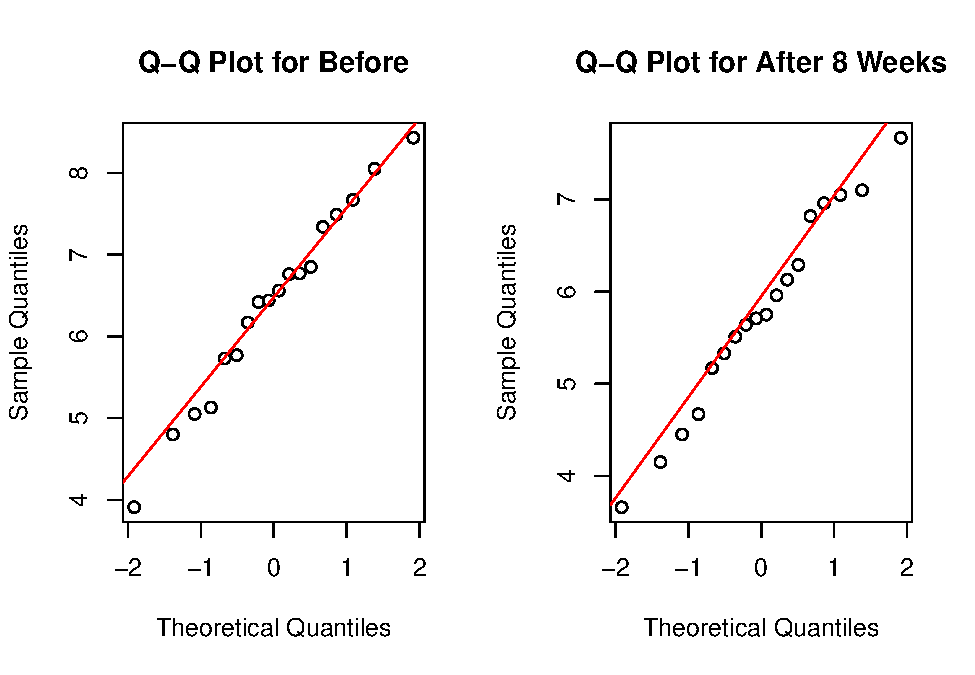
\includegraphics{ReportAssignment1_files/figure-latex/unnamed-chunk-3-1.pdf}

To further explore the normality assumption, histograms below are
plotted for both \emph{Before} and \emph{After8weeks}. The histograms
exhibit a roughly bell-shaped distribution, which supports the
assumption of normality.

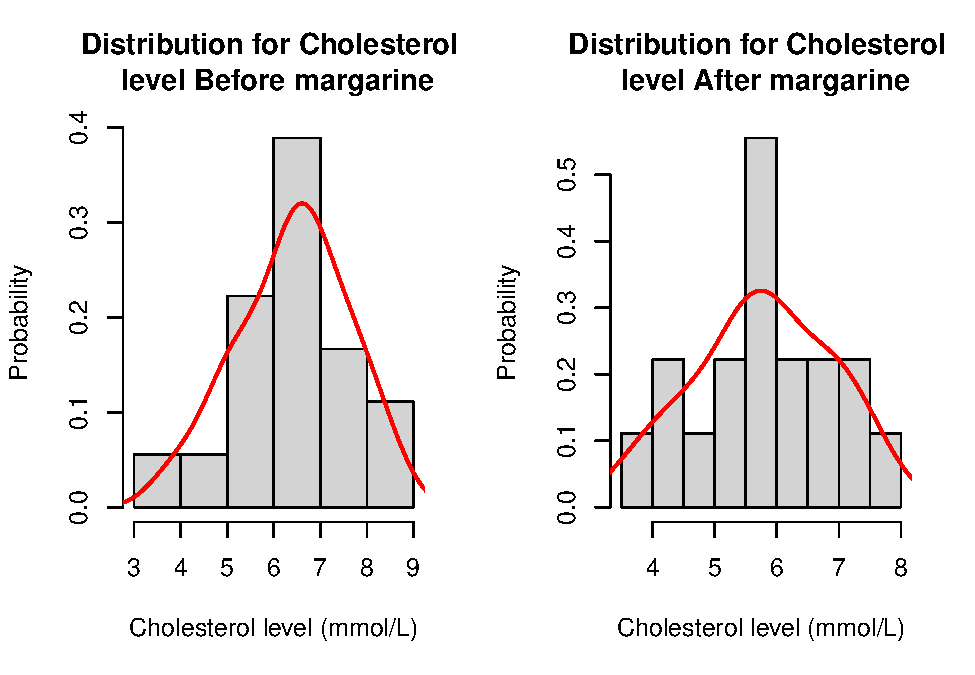
\includegraphics{ReportAssignment1_files/figure-latex/unnamed-chunk-4-1.pdf}

However, to address normality more formally, a Shapiro-Wilk test is
conducted, as this test is suitable to test for normality for small data
sets. The null hypothesis is as follows:

H0: The data is normally distributed.

The W-statistic measures how closely the data aligns with a normal
distribution, ranging from 0 to 1, where values closer to 1 indicate a
stronger likelihood of normality. Considering the results for
\emph{Before} and \emph{After8weeks}, both W-values are close to 1.
Additionally, with a 95\% confidence level, both p-values exceed 0.05,
meaning that we fail to reject H0. These findings provide strong
evidence that the data in both columns can be considered to be normally
distributed.

\begin{Shaded}
\begin{Highlighting}[]
\NormalTok{shapiro\_before }\OtherTok{=} \FunctionTok{shapiro.test}\NormalTok{(data}\SpecialCharTok{$}\NormalTok{Before)}
\NormalTok{shapiro\_after }\OtherTok{=} \FunctionTok{shapiro.test}\NormalTok{(data}\SpecialCharTok{$}\NormalTok{After8weeks)}
\end{Highlighting}
\end{Shaded}

\begin{verbatim}
## Shapiro-Wilk Test for Before:
\end{verbatim}

\begin{verbatim}
## W-statistic = 0.982 , p-value = 0.967
\end{verbatim}

\begin{verbatim}
## Shapiro-Wilk Test for After 8 Weeks:
\end{verbatim}

\begin{verbatim}
## W-statistic = 0.982 , p-value = 0.918
\end{verbatim}

In order to investigate the relationship between the columns of
\emph{Before} and \emph{After8weeks} a scatter plot is created below.
The scatter plot demonstrates a strong positive correlation between
`Before' and `After8weeks' cholesterol levels. The data points align
closely with the red regression line, suggesting that individuals with
higher cholesterol levels before the diet intervention also tend to have
higher cholesterol levels after 8 weeks. This indicates that while
cholesterol levels may have decreased, there remains a strong
relationship between pre- and post-diet measurements.

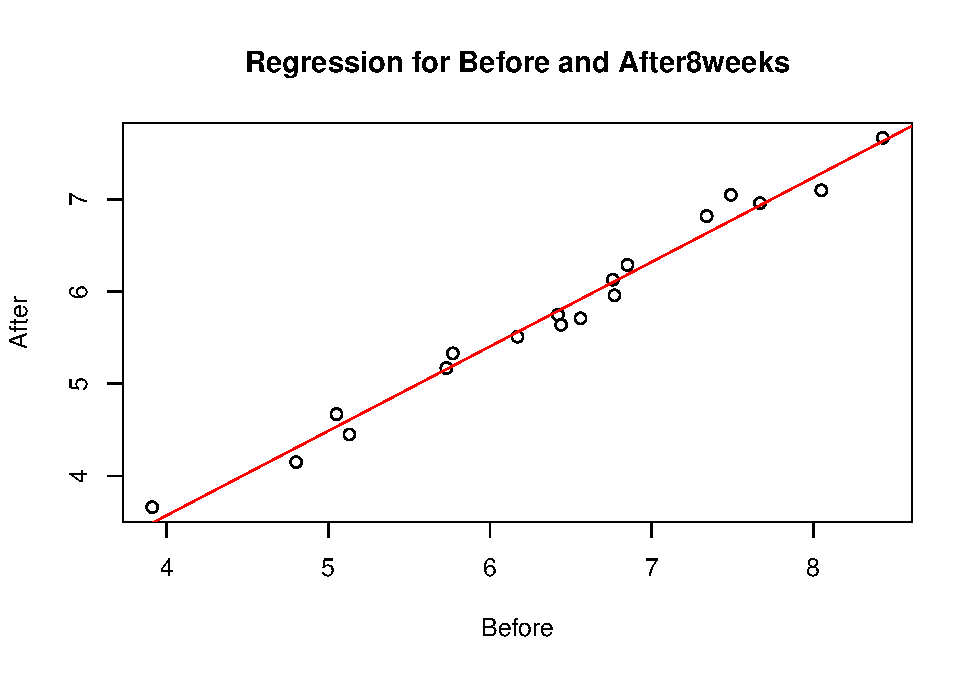
\includegraphics{ReportAssignment1_files/figure-latex/unnamed-chunk-7-1.pdf}

To quantify this correlation, the Pearson's correlation coefficient is
calculated below. A high Pearson correlation (close to 1) indicates a
strong positive relationship between the two columns. The correlation
coefficient exhibits a value of approximately 0.99, confirming the
strong positive relationship. Additionally, the p-value is smaller than
0.05, indicating that the correlation is statistically significant.

\begin{Shaded}
\begin{Highlighting}[]
\NormalTok{cor\_result }\OtherTok{=} \FunctionTok{cor.test}\NormalTok{(data}\SpecialCharTok{$}\NormalTok{Before, data}\SpecialCharTok{$}\NormalTok{After8weeks, }\AttributeTok{method =} \StringTok{"pearson"}\NormalTok{)}
\end{Highlighting}
\end{Shaded}

\begin{verbatim}
## Pearson Correlation Test:
\end{verbatim}

\begin{verbatim}
## Correlation coefficient (r) =  0.991 p-value = 2.321e-15
\end{verbatim}

\begin{verbatim}
## 95% Confidence Interval: [ 0.975 , 0.997 ]
\end{verbatim}

\paragraph{Section b}\label{section-b}

As the cholesterol data was measured on the same population at different
times, we consider the data to be paired. In this case it is possible to
conduct a T-test for paired samples. However, as the T-test assumes a
normal distribution for the mean difference, we have to check whether
this is the case first.

The histogram suggests a roughly bell-shaped distribution, with the
density curve closely following the bars, supporting the assumption of
normality. The data are centered around 0.6--0.7, indicating an average
decrease in cholesterol levels after 8 weeks. The Q-Q plot shows that
the data points align well with the diagonal red line, further
suggesting an approximate normal distribution, though slight deviations
in the lower left tail may indicate mild skewness. However, given the
small sample size (n = 18), such variability is expected and does not
suggest a major departure from normality, making parametric tests like
the paired t-test reasonable.

\includegraphics{ReportAssignment1_files/figure-latex/unnamed-chunk-10-1.pdf}

To assess whether the mean difference is normally distributed for the
t-test, a Shapiro-Wilk test is conducted:

H0: The data is normally distributed.

The W-statistic (≈ 0.99) is close to 1, and the p-value exceeds 0.05,
meaning we fail to reject H0, providing strong evidence that the mean
difference follows a normal distribution.

\begin{Shaded}
\begin{Highlighting}[]
\NormalTok{difference }\OtherTok{=}\NormalTok{ data}\SpecialCharTok{$}\NormalTok{Before }\SpecialCharTok{{-}}\NormalTok{ data}\SpecialCharTok{$}\NormalTok{After8weeks}
\NormalTok{shapiro\_result }\OtherTok{=} \FunctionTok{shapiro.test}\NormalTok{(difference)}
\end{Highlighting}
\end{Shaded}

\begin{verbatim}
## Shapiro-Wilk Test for Mean Difference:
\end{verbatim}

\begin{verbatim}
## W-statistic = 0.985 , p-value = 0.987
\end{verbatim}

Since we have strong evidence to assume that the data is normally
distributed, we can proceed to conduct the T-test. For this, we consider
the following null hypothesis:

H0: The margarine diet has no effect, i.e.~the mean cholesterol levels
\emph{Before} and \emph{After8weeks} are the same.

The paired t-test results show a t-statistic of 14.946 with 17 degrees
of freedom and an extremely small p-value (1.639e-11), providing strong
evidence to reject the null hypothesis. This supports the alternative
hypothesis that the true mean difference is greater than 0, indicating
that cholesterol levels were significantly lower after 8 weeks on the
margarine diet. The mean difference of 0.629 mmol/L further reinforces
this conclusion, showing an average reduction in cholesterol.
Additionally, the 95\% confidence interval {[}0.556, ∞{]} suggests that
the true mean reduction is at least 0.556 mmol/L, with the infinite
upper bound resulting from the one-sided test.

\begin{Shaded}
\begin{Highlighting}[]
\NormalTok{t\_test\_result }\OtherTok{=} \FunctionTok{t.test}\NormalTok{(data}\SpecialCharTok{$}\NormalTok{Before, data}\SpecialCharTok{$}\NormalTok{After8weeks, }\AttributeTok{paired =} \ConstantTok{TRUE}\NormalTok{, }\AttributeTok{alternative =} \StringTok{"greater"}\NormalTok{)}
\end{Highlighting}
\end{Shaded}

\begin{verbatim}
## Paired T-Test Results:
\end{verbatim}

\begin{verbatim}
## T-statistic = 14.946 , p-value = 1.639e-11
\end{verbatim}

\begin{verbatim}
## 95% Confidence Interval: [ 0.556 , Inf ]
\end{verbatim}

The permutation test was conducted to assess whether there is a
significant difference between cholesterol levels before and after 8
weeks on the margarine diet. The observed mean difference is 0.629
mmol/L, and the permutation test p-value is 1.0e-05, which is extremely
small. This provides strong evidence to reject the null hypothesis,
confirming that the margarine diet had a significant effect on reducing
cholesterol levels.

It is not possible to apply a Mann-Whitney U-test as the data is paired,
and this test is only for independent samples.

\begin{Shaded}
\begin{Highlighting}[]
\NormalTok{diff }\OtherTok{=}\NormalTok{ data}\SpecialCharTok{$}\NormalTok{Before }\SpecialCharTok{{-}}\NormalTok{ data}\SpecialCharTok{$}\NormalTok{After8weeks}
\NormalTok{n\_permutations }\OtherTok{=} \DecValTok{100000}
\NormalTok{observed\_mean }\OtherTok{=} \FunctionTok{mean}\NormalTok{(diff)}

\NormalTok{permute\_test }\OtherTok{=} \ControlFlowTok{function}\NormalTok{(diff) \{}
\NormalTok{  permuted\_diff }\OtherTok{\textless{}{-}}\NormalTok{ diff }\SpecialCharTok{*} \FunctionTok{sample}\NormalTok{(}\FunctionTok{c}\NormalTok{(}\SpecialCharTok{{-}}\DecValTok{1}\NormalTok{, }\DecValTok{1}\NormalTok{), }\FunctionTok{length}\NormalTok{(diff), }\AttributeTok{replace =} \ConstantTok{TRUE}\NormalTok{)}
  \FunctionTok{return}\NormalTok{(}\FunctionTok{mean}\NormalTok{(permuted\_diff)) }
\NormalTok{\}}

\FunctionTok{set.seed}\NormalTok{(}\DecValTok{42}\NormalTok{)}
\NormalTok{permute\_distr }\OtherTok{=} \FunctionTok{replicate}\NormalTok{(n\_permutations, }\FunctionTok{permute\_test}\NormalTok{(diff))}
\NormalTok{rounded\_observed\_mean }\OtherTok{=} \FunctionTok{round}\NormalTok{(observed\_mean, }\DecValTok{3}\NormalTok{) }
\NormalTok{rounded\_p\_value }\OtherTok{=} \FunctionTok{formatC}\NormalTok{(}\FunctionTok{mean}\NormalTok{(}\FunctionTok{abs}\NormalTok{(permute\_distr) }\SpecialCharTok{\textgreater{}=} \FunctionTok{abs}\NormalTok{(observed\_mean)), }\AttributeTok{format =} \StringTok{"e"}\NormalTok{, }\AttributeTok{digits =} \DecValTok{3}\NormalTok{)}
\FunctionTok{cat}\NormalTok{(}\StringTok{"Observed mean difference:"}\NormalTok{, rounded\_observed\_mean, }\StringTok{"}\SpecialCharTok{\textbackslash{}n}\StringTok{"}\NormalTok{)}
\end{Highlighting}
\end{Shaded}

\begin{verbatim}
## Observed mean difference: 0.629
\end{verbatim}

\begin{Shaded}
\begin{Highlighting}[]
\FunctionTok{cat}\NormalTok{(}\StringTok{"Permutation test p{-}value:"}\NormalTok{, rounded\_p\_value)}
\end{Highlighting}
\end{Shaded}

\begin{verbatim}
## Permutation test p-value: 1.000e-05
\end{verbatim}

\paragraph{Section c}\label{section-c}

To construct a 97\% confidence interval for the mean cholesterol level
after 8 weeks, we first calculate the sample mean (5.77) and sample
standard deviation (1.11). Using the t-distribution with 17 degrees of
freedom, we obtain a 97\% CI of {[}5.164, 6.394{]}.

Since bootstrapping does not assume normality, we also compute a
bootstrap 97\% CI, resampling the data 10,000 times and taking the 1.5\%
and 98.5\% percentiles, resulting in {[}5.230, 6.320{]}. The substantial
overlap between the t-test and bootstrap CIs suggests that both methods
provide similar estimates for the mean. The slight differences arise
because the t-test assumes normality, while bootstrapping relies purely
on resampling. Since both methods lead to consistent results, this
reinforces confidence that the true mean cholesterol level falls within
this range. Overall, the findings suggest that cholesterol levels remain
moderate after 8 weeks on the diet.

\begin{Shaded}
\begin{Highlighting}[]
\CommentTok{\# calculating 97\% CI for mu using t{-}score}
\NormalTok{n }\OtherTok{=} \FunctionTok{length}\NormalTok{(data}\SpecialCharTok{$}\NormalTok{After8weeks)}
\NormalTok{sample\_mean }\OtherTok{=} \FunctionTok{mean}\NormalTok{(data}\SpecialCharTok{$}\NormalTok{After8weeks)}
\NormalTok{sample\_sd }\OtherTok{=} \FunctionTok{sd}\NormalTok{(data}\SpecialCharTok{$}\NormalTok{After8weeks)}
\NormalTok{critical\_value }\OtherTok{=} \FunctionTok{qt}\NormalTok{(}\DecValTok{1}\FloatTok{{-}0.015}\NormalTok{, }\AttributeTok{df=}\DecValTok{17}\NormalTok{)}
\NormalTok{standard\_error }\OtherTok{=}\NormalTok{ sample\_sd }\SpecialCharTok{/} \FunctionTok{sqrt}\NormalTok{(n)}

\NormalTok{left\_bound }\OtherTok{=}\NormalTok{ sample\_mean }\SpecialCharTok{{-}}\NormalTok{ critical\_value }\SpecialCharTok{*}\NormalTok{ standard\_error}
\NormalTok{right\_bound }\OtherTok{=}\NormalTok{ sample\_mean }\SpecialCharTok{+}\NormalTok{ critical\_value }\SpecialCharTok{*}\NormalTok{ standard\_error}

\CommentTok{\# calculating 97\% CI for mu with bootstrapping}
\NormalTok{bootstrap\_ci }\OtherTok{=} \ControlFlowTok{function}\NormalTok{(x, }\AttributeTok{conf\_level =} \FloatTok{0.97}\NormalTok{, }\AttributeTok{B =} \DecValTok{10000}\NormalTok{) \{}
\NormalTok{  alpha }\OtherTok{=} \DecValTok{1} \SpecialCharTok{{-}}\NormalTok{ conf\_level}
\NormalTok{  Bstats }\OtherTok{=} \FunctionTok{lapply}\NormalTok{(}\DecValTok{1}\SpecialCharTok{:}\NormalTok{B, }\AttributeTok{FUN =} \ControlFlowTok{function}\NormalTok{(i) \{}
\NormalTok{    boot\_sample }\OtherTok{=} \FunctionTok{sample}\NormalTok{(x, }\AttributeTok{size =} \FunctionTok{length}\NormalTok{(x), }\AttributeTok{replace =} \ConstantTok{TRUE}\NormalTok{)}
    \FunctionTok{mean}\NormalTok{(boot\_sample)}
\NormalTok{  \} )}
\NormalTok{  Bstats }\OtherTok{=} \FunctionTok{unlist}\NormalTok{(Bstats)}
\NormalTok{  ci }\OtherTok{=} \FunctionTok{round}\NormalTok{(}\FunctionTok{quantile}\NormalTok{(Bstats, }\AttributeTok{prob =} \FunctionTok{c}\NormalTok{(alpha}\SpecialCharTok{/}\DecValTok{2}\NormalTok{, }\DecValTok{1}\SpecialCharTok{{-}}\NormalTok{alpha}\SpecialCharTok{/}\DecValTok{2}\NormalTok{)), }\DecValTok{3}\NormalTok{)}
  \FunctionTok{cat}\NormalTok{(}\StringTok{"Bootstrap test with"}\NormalTok{, conf\_level }\SpecialCharTok{*} \DecValTok{100}\NormalTok{, }\StringTok{"\% Confidence Interval:}\SpecialCharTok{\textbackslash{}n}\StringTok{"}\NormalTok{)}
  \FunctionTok{return}\NormalTok{ (ci)}
\NormalTok{\}}
\end{Highlighting}
\end{Shaded}

\begin{verbatim}
## The sample mean is: 5.779
\end{verbatim}

\begin{verbatim}
## The sample standard deviation is: 1.102
\end{verbatim}

\begin{verbatim}
## The critical value is: 2.368
\end{verbatim}

\begin{verbatim}
## 97% Confidence Interval for mu: [ 5.164 , 6.394 ]
\end{verbatim}

\begin{verbatim}
## Bootstrap test with 97 % Confidence Interval:
\end{verbatim}

\begin{verbatim}
##  1.5% 98.5% 
##  5.23  6.32
\end{verbatim}

\paragraph{Section d}\label{section-d}

For the bootstrap test, we consider the following null hypothesis:

H0: The data follows a uniform distribution with a minimum of 3 and a
maximum of θ.

To generate bootstrap samples from a Uniform(3, θ) distribution, we
iterate over θ values from 3 to 12 in steps of 1, generating 100,000
bootstrap samples for each. The maximum value from each re-sample is
recorded, and the p-value is computed by comparing the observed
maximum(\emph{T\_max\_observed}) with the bootstrap distribution
(\emph{t\_star}).

\begin{Shaded}
\begin{Highlighting}[]
\FunctionTok{set.seed}\NormalTok{(}\DecValTok{42}\NormalTok{) }\CommentTok{\# ensure reproducability}

\NormalTok{T\_max\_observed }\OtherTok{=} \FunctionTok{max}\NormalTok{(data}\SpecialCharTok{$}\NormalTok{After8weeks)}
\NormalTok{n }\OtherTok{=} \FunctionTok{length}\NormalTok{(data}\SpecialCharTok{$}\NormalTok{After8weeks)}

\ControlFlowTok{for}\NormalTok{ (theta }\ControlFlowTok{in} \DecValTok{3}\SpecialCharTok{:}\DecValTok{12}\NormalTok{) \{}
\NormalTok{  Bootstraps }\OtherTok{=} \DecValTok{100000}  
\NormalTok{  t\_star }\OtherTok{=} \FunctionTok{numeric}\NormalTok{(Bootstraps)  }
  
  \ControlFlowTok{for}\NormalTok{ (i }\ControlFlowTok{in} \DecValTok{1}\SpecialCharTok{:}\NormalTok{Bootstraps) \{}
\NormalTok{    x\_star }\OtherTok{=} \FunctionTok{runif}\NormalTok{(n, }\AttributeTok{min =} \DecValTok{3}\NormalTok{, }\AttributeTok{max =}\NormalTok{ theta) }
\NormalTok{    t\_star[i] }\OtherTok{=} \FunctionTok{max}\NormalTok{(x\_star)}
\NormalTok{  \}}
  
\NormalTok{  pl }\OtherTok{=} \FunctionTok{sum}\NormalTok{(t\_star }\SpecialCharTok{\textless{}}\NormalTok{ T\_max\_observed) }\SpecialCharTok{/}\NormalTok{ Bootstraps  }
\NormalTok{  pr }\OtherTok{=} \FunctionTok{sum}\NormalTok{(t\_star }\SpecialCharTok{\textgreater{}}\NormalTok{ T\_max\_observed) }\SpecialCharTok{/}\NormalTok{ Bootstraps  }
\NormalTok{  p }\OtherTok{=} \DecValTok{2} \SpecialCharTok{*} \FunctionTok{min}\NormalTok{(pl, pr)}

  \FunctionTok{print}\NormalTok{(}\FunctionTok{paste}\NormalTok{(}\StringTok{"Theta ="}\NormalTok{, theta, }\StringTok{", p{-}value ="}\NormalTok{, }\FunctionTok{round}\NormalTok{(p, }\DecValTok{3}\NormalTok{)))}
\NormalTok{\}}
\end{Highlighting}
\end{Shaded}

\begin{verbatim}
## [1] "Theta = 3 , p-value = 0"
## [1] "Theta = 4 , p-value = 0"
## [1] "Theta = 5 , p-value = 0"
## [1] "Theta = 6 , p-value = 0"
## [1] "Theta = 7 , p-value = 0"
## [1] "Theta = 8 , p-value = 0.58"
## [1] "Theta = 9 , p-value = 0.021"
## [1] "Theta = 10 , p-value = 0.001"
## [1] "Theta = 11 , p-value = 0"
## [1] "Theta = 12 , p-value = 0"
\end{verbatim}

To generate bootstrap samples from a Uniform(3, θ) distribution, we
iterate over θ values from 3 to 12 in steps of 1, generating 100,000
bootstrap samples for each. The maximum value from each re-sample is
recorded, and the p-value is computed by comparing the observed
maximum(\emph{T\_max\_observed}) with the bootstrap distribution
(\emph{t\_star}).

\begin{Shaded}
\begin{Highlighting}[]
\NormalTok{accepted\_theta }\OtherTok{\textless{}{-}} \FunctionTok{c}\NormalTok{(}\DecValTok{8}\NormalTok{, }\DecValTok{9}\NormalTok{, }\DecValTok{10}\NormalTok{, }\DecValTok{11}\NormalTok{)}

\ControlFlowTok{for}\NormalTok{ (theta }\ControlFlowTok{in}\NormalTok{ accepted\_theta) \{}
\NormalTok{  ks\_test\_result }\OtherTok{\textless{}{-}} \FunctionTok{ks.test}\NormalTok{(data}\SpecialCharTok{$}\NormalTok{After8weeks, }\StringTok{"punif"}\NormalTok{, }\AttributeTok{min =} \DecValTok{3}\NormalTok{, }\AttributeTok{max =}\NormalTok{ theta)}

\NormalTok{  rounded\_statistic }\OtherTok{\textless{}{-}} \FunctionTok{round}\NormalTok{(ks\_test\_result}\SpecialCharTok{$}\NormalTok{statistic, }\DecValTok{3}\NormalTok{)}
\NormalTok{  rounded\_p\_value }\OtherTok{\textless{}{-}} \FunctionTok{formatC}\NormalTok{(ks\_test\_result}\SpecialCharTok{$}\NormalTok{p.value, }\AttributeTok{format =} \StringTok{"e"}\NormalTok{, }\AttributeTok{digits =} \DecValTok{3}\NormalTok{)}
  \FunctionTok{cat}\NormalTok{(}\StringTok{"}\SpecialCharTok{\textbackslash{}n}\StringTok{Kolmogorov{-}Smirnov Test for Uniform(3,"}\NormalTok{, theta, }\StringTok{"):}\SpecialCharTok{\textbackslash{}n}\StringTok{"}\NormalTok{)}
  \FunctionTok{cat}\NormalTok{(}\StringTok{"D{-}statistic:"}\NormalTok{, rounded\_statistic, }\StringTok{"}\SpecialCharTok{\textbackslash{}n}\StringTok{"}\NormalTok{)}
  \FunctionTok{cat}\NormalTok{(}\StringTok{"P{-}value:"}\NormalTok{, rounded\_p\_value, }\StringTok{"}\SpecialCharTok{\textbackslash{}n}\StringTok{"}\NormalTok{)}
\NormalTok{\}}
\end{Highlighting}
\end{Shaded}

\begin{verbatim}
## 
## Kolmogorov-Smirnov Test for Uniform(3, 8 ):
## D-statistic: 0.212 
## P-value: 3.451e-01 
## 
## Kolmogorov-Smirnov Test for Uniform(3, 9 ):
## D-statistic: 0.261 
## P-value: 1.429e-01 
## 
## Kolmogorov-Smirnov Test for Uniform(3, 10 ):
## D-statistic: 0.359 
## P-value: 1.401e-02 
## 
## Kolmogorov-Smirnov Test for Uniform(3, 11 ):
## D-statistic: 0.432 
## P-value: 1.438e-03
\end{verbatim}

For θ = 9, θ = 10, and θ = 11 we get a p-value \textless{} 0.05, thus we
reject H0 indicating that the observed maximum for these values is
significantly different from the expected maximum under U(3,θ). For θ =
8, we fail to reject H0, meaning that the data could be from a uniform
distribution.

\paragraph{Section e}\label{section-e}

To test whether the median of the cholesterol level is less than 6, we
will use a Wilcoxon signed-rank test, because it is a non-parametric
test that does not assume normality, making it suitable for small sample
sizes and skewed data. The null hypothesis is:

H0: The median cholesterol level is 6 or greater.

The test yields a p-value of 0.223, meaning we fail to reject
H0\hspace{0pt}. This suggests that the median cholesterol level after 8
weeks is not significantly less than 6 at the 5\% significance level.

\begin{Shaded}
\begin{Highlighting}[]
\FunctionTok{wilcox.test}\NormalTok{(data}\SpecialCharTok{$}\NormalTok{After8weeks, }\AttributeTok{mu =} \DecValTok{6}\NormalTok{, }\AttributeTok{alternative =} \StringTok{"less"}\NormalTok{, }\AttributeTok{exact =} \ConstantTok{FALSE}\NormalTok{)}
\end{Highlighting}
\end{Shaded}

\begin{verbatim}
## 
##  Wilcoxon signed rank test with continuity correction
## 
## data:  data$After8weeks
## V = 67.5, p-value = 0.223
## alternative hypothesis: true location is less than 6
\end{verbatim}

To determine whether the fraction of cholesterol levels below 4.5 after
8 weeks exceeds 25\%, a binomial test is conducted. The null hypothesis
is:

H0: The fraction of cholesterol levels below 4.5 is at most 25\%.

The test yields a p-value of 0.865, meaning we fail to reject
H0\hspace{0pt} at the 5\% significance level. This suggests that there
is no significant evidence that the proportion of cholesterol levels
below 4.5 is greater than 25\%.

\begin{Shaded}
\begin{Highlighting}[]
\NormalTok{count\_below\_4}\FloatTok{.5} \OtherTok{=} \FunctionTok{sum}\NormalTok{(data}\SpecialCharTok{$}\NormalTok{After8weeks }\SpecialCharTok{\textless{}} \FloatTok{4.5}\NormalTok{)}
\NormalTok{binom\_result }\OtherTok{=} \FunctionTok{binom.test}\NormalTok{(count\_below\_4}\FloatTok{.5}\NormalTok{, }\FunctionTok{length}\NormalTok{(data}\SpecialCharTok{$}\NormalTok{After8weeks), }\AttributeTok{p =} \FloatTok{0.25}\NormalTok{, }\AttributeTok{alternative =} \StringTok{"greater"}\NormalTok{)}
\end{Highlighting}
\end{Shaded}

\begin{verbatim}
## Exact binomial test
\end{verbatim}

\begin{verbatim}
## Number of successes: 3
\end{verbatim}

\begin{verbatim}
## Number of trials: 18
\end{verbatim}

\begin{verbatim}
## P-value: 0.865
\end{verbatim}

\begin{verbatim}
## 95% Confidence Interval: [ 0.047 1 ]
\end{verbatim}

\begin{verbatim}
## Estimated probability of success: 0.167
\end{verbatim}

\subsection{Exercise 2: Crops}\label{exercise-2-crops}

First we load the necessary data

\begin{Shaded}
\begin{Highlighting}[]
\NormalTok{  crops\_data }\OtherTok{\textless{}{-}} \FunctionTok{read.table}\NormalTok{(}\StringTok{"crops.txt"}\NormalTok{, }\AttributeTok{header=}\ConstantTok{TRUE}\NormalTok{)}
\NormalTok{  crops\_data}\SpecialCharTok{$}\NormalTok{County }\OtherTok{\textless{}{-}} \FunctionTok{as.factor}\NormalTok{(crops\_data}\SpecialCharTok{$}\NormalTok{County)         }
\NormalTok{  crops\_data}\SpecialCharTok{$}\NormalTok{Related }\OtherTok{\textless{}{-}} \FunctionTok{as.factor}\NormalTok{(crops\_data}\SpecialCharTok{$}\NormalTok{Related)}
\end{Highlighting}
\end{Shaded}

\subsubsection{Section a}\label{section-a-1}

We want to investigate whether two factors County and Related (and
possibly their interaction) influence the crops by performing relevant
ANOVA model(s), without taking Size into account. So we create and test
3 separate Null Hypotheses with a two-way ANOVA: H\_(01): There is no
significant difference in the mean Crops yield across different
Counties. (the means of observations grouped by country are the same)
H\_(02): There is no significant difference in the mean Crops yield
between cases where the landlord and tenant are related versus not
related. (the means of observations grouped by related are the same)
H\_(03): There is no interaction effect between County and Related on
Crops yield (there is no interaction between county and related)

\begin{Shaded}
\begin{Highlighting}[]
\NormalTok{model\_a }\OtherTok{\textless{}{-}} \FunctionTok{lm}\NormalTok{(Crops }\SpecialCharTok{\textasciitilde{}}\NormalTok{ County }\SpecialCharTok{*}\NormalTok{ Related, }\AttributeTok{data =}\NormalTok{ crops\_data)}
\FunctionTok{anova}\NormalTok{(model\_a)}
\end{Highlighting}
\end{Shaded}

\begin{verbatim}
## Analysis of Variance Table
## 
## Response: Crops
##                Df    Sum Sq Mean Sq F value Pr(>F)
## County          2   8841441 4420721  0.7644 0.4766
## Related         1   2378957 2378957  0.4113 0.5274
## County:Related  2   1497573  748786  0.1295 0.8792
## Residuals      24 138805865 5783578
\end{verbatim}

From this table we can see the following: For County:The p-value (0.476)
is greater than 0.05, meaning we fail to reject the null hypothesis
H\_(01), suggesting that there is no significant effect of the County on
the Crops variable. For related: The p-value (0.527) is also greater
than 0.05, meaning we fail to reject the null hypothesis H\_(02), which
means that there is no significant effect of whether the landlord and
tenant are related on the Crops variable. For both: The p-value (0.879)
is much greater than 0.05, meaning we fail to reject the null hypothesis
H\_(03), implying there is no significant interaction between County and
Related on the Crops variable.

\begin{Shaded}
\begin{Highlighting}[]
\FunctionTok{summary}\NormalTok{(model\_a)}
\end{Highlighting}
\end{Shaded}

\begin{verbatim}
## 
## Call:
## lm(formula = Crops ~ County * Related, data = crops_data)
## 
## Residuals:
##     Min      1Q  Median      3Q     Max 
## -3120.4 -1744.7  -176.9  2064.2  4806.6 
## 
## Coefficients:
##                    Estimate Std. Error t value Pr(>|t|)    
## (Intercept)          6700.0     1075.5   6.230 1.94e-06 ***
## County2                93.0     1521.0   0.061    0.952    
## County3               851.2     1521.0   0.560    0.581    
## Relatedyes           -362.0     1521.0  -0.238    0.814    
## County2:Relatedyes   -820.6     2151.0  -0.381    0.706    
## County3:Relatedyes    217.0     2151.0   0.101    0.920    
## ---
## Signif. codes:  0 '***' 0.001 '**' 0.01 '*' 0.05 '.' 0.1 ' ' 1
## 
## Residual standard error: 2405 on 24 degrees of freedom
## Multiple R-squared:  0.08393,    Adjusted R-squared:  -0.1069 
## F-statistic: 0.4398 on 5 and 24 DF,  p-value: 0.8163
\end{verbatim}

The above model summary table aligns with the ANOVA p-values as both
show that none of the predictors(County, Related, or their interaction)
are significant in either table.

\includegraphics{ReportAssignment1_files/figure-latex/unnamed-chunk-26-1.pdf}

While the above plots suggests potential interaction effects
(non-parallel lines), statistical analysis via ANOVA and linear
regression indicates that these differences are not statistically
significant (p \textgreater{} 0.05). This suggests that observed
variations in the plot may be due to random noise rather than meaningful
effects of County or Related on Crops.

Finally, we have to check the model assumptions

\includegraphics{ReportAssignment1_files/figure-latex/unnamed-chunk-27-1.pdf}

\includegraphics{ReportAssignment1_files/figure-latex/unnamed-chunk-28-1.pdf}

\begin{Shaded}
\begin{Highlighting}[]
\FunctionTok{round}\NormalTok{(}\FunctionTok{shapiro.test}\NormalTok{(}\FunctionTok{residuals}\NormalTok{(model\_a))}\SpecialCharTok{$}\NormalTok{p.value, }\DecValTok{3}\NormalTok{)}
\end{Highlighting}
\end{Shaded}

\begin{verbatim}
## [1] 0.099
\end{verbatim}

\begin{Shaded}
\begin{Highlighting}[]
\FunctionTok{round}\NormalTok{(}\FunctionTok{shapiro.test}\NormalTok{(}\FunctionTok{residuals}\NormalTok{(model\_a))}\SpecialCharTok{$}\NormalTok{statistic, }\DecValTok{3}\NormalTok{)}
\end{Highlighting}
\end{Shaded}

\begin{verbatim}
##     W 
## 0.941
\end{verbatim}

The Q-Q plot shows minor deviations from normality, particularly in the
tails, but the overall trend follows the theoretical quantiles. The
residuals vs.~fitted plot suggests no strong patterns, indicating an
approximately random distribution of residuals. Given the small sample
size (n = 30), results should be interpreted with caution, as minor
departures from normality can impact statistical inference.The
Shapiro-Wilk test (W = 0.941, p = 0.099) fails to reject the null
hypothesis of normality at the 0.05 level.

We estimate the crops for County 3 when landlord and tenant are not
related We implement 2 different ways of the prediction First way: We
computes the raw mean of Crops for the subset of data where the County
is ``3'' and the Related is ``no''. This doesn't account for any
potential modeling (such as an interaction effect) or covariates and is
a straightforward group mean estimate.

\begin{Shaded}
\begin{Highlighting}[]
\NormalTok{predicted\_value }\OtherTok{\textless{}{-}} \FunctionTok{with}\NormalTok{(crops\_data, }\FunctionTok{mean}\NormalTok{(Crops[County }\SpecialCharTok{==} \StringTok{"3"} \SpecialCharTok{\&}\NormalTok{ Related }\SpecialCharTok{==} \StringTok{"no"}\NormalTok{], }\AttributeTok{na.rm=}\ConstantTok{TRUE}\NormalTok{))}
\FunctionTok{cat}\NormalTok{(}\StringTok{"Estimated crops for County 3 (Landlord and Tenant NOT related):"}\NormalTok{, predicted\_value, }\StringTok{"}\SpecialCharTok{\textbackslash{}n}\StringTok{"}\NormalTok{)}
\end{Highlighting}
\end{Shaded}

\begin{verbatim}
## Estimated crops for County 3 (Landlord and Tenant NOT related): 7551.2
\end{verbatim}

Second way: We use the emmeans function to estimate the adjusted mean
crops yield for a typical farm in County 3 where the landlord and tenant
are not related, based on the fitted linear model (anova\_model). The
emmeans function provides the estimated marginal means, which account
for the effects of the factors (County and Related) while adjusting for
any interactions.

\begin{Shaded}
\begin{Highlighting}[]
\NormalTok{emm\_results }\OtherTok{\textless{}{-}}\NormalTok{ emmeans}\SpecialCharTok{::}\FunctionTok{emmeans}\NormalTok{(model\_a, }\SpecialCharTok{\textasciitilde{}}\NormalTok{ County }\SpecialCharTok{*}\NormalTok{ Related)}
\NormalTok{emm\_summary }\OtherTok{\textless{}{-}} \FunctionTok{as.data.frame}\NormalTok{(emm\_results)}
\NormalTok{county3\_not\_related }\OtherTok{\textless{}{-}}\NormalTok{ emm\_summary[emm\_summary}\SpecialCharTok{$}\NormalTok{County }\SpecialCharTok{==} \StringTok{"3"} \SpecialCharTok{\&}\NormalTok{ emm\_summary}\SpecialCharTok{$}\NormalTok{Related }\SpecialCharTok{==} \StringTok{"no"}\NormalTok{, ]}
\FunctionTok{cat}\NormalTok{(}\StringTok{"Estimated crops for County 3 (Landlord and Tenant NOT related):"}\NormalTok{, county3\_not\_related}\SpecialCharTok{$}\NormalTok{emmean, }\StringTok{"}\SpecialCharTok{\textbackslash{}n}\StringTok{"}\NormalTok{)}
\end{Highlighting}
\end{Shaded}

\begin{verbatim}
## Estimated crops for County 3 (Landlord and Tenant NOT related): 7551.2
\end{verbatim}

\subsubsection{Section b}\label{section-b-1}

First, we ensure correct formatting of the data

\begin{Shaded}
\begin{Highlighting}[]
\NormalTok{crops\_data}\SpecialCharTok{$}\NormalTok{County }\OtherTok{\textless{}{-}} \FunctionTok{as.factor}\NormalTok{(crops\_data}\SpecialCharTok{$}\NormalTok{County)}
\NormalTok{crops\_data}\SpecialCharTok{$}\NormalTok{Related }\OtherTok{\textless{}{-}} \FunctionTok{as.factor}\NormalTok{(crops\_data}\SpecialCharTok{$}\NormalTok{Related)}
\NormalTok{crops\_data}\SpecialCharTok{$}\NormalTok{Size }\OtherTok{\textless{}{-}} \FunctionTok{as.numeric}\NormalTok{(crops\_data}\SpecialCharTok{$}\NormalTok{Size) }
\NormalTok{crops\_data}\SpecialCharTok{$}\NormalTok{Crops }\OtherTok{\textless{}{-}} \FunctionTok{as.numeric}\NormalTok{(crops\_data}\SpecialCharTok{$}\NormalTok{Crops)}
\end{Highlighting}
\end{Shaded}

We define 3 different models: Model\_county\_size: This model examines
how crop yields are influenced by County, Related, and Size, with an
additional focus on the interaction between County and Size. It does not
include an interaction term for Related.

\begin{Shaded}
\begin{Highlighting}[]
\NormalTok{model\_county\_size }\OtherTok{\textless{}{-}} \FunctionTok{lm}\NormalTok{(Crops }\SpecialCharTok{\textasciitilde{}}\NormalTok{ Size }\SpecialCharTok{*}\NormalTok{ County }\SpecialCharTok{+}\NormalTok{ Related, }\AttributeTok{data =}\NormalTok{ crops\_data)}
\FunctionTok{anova}\NormalTok{(model\_county\_size)}
\end{Highlighting}
\end{Shaded}

\begin{verbatim}
## Analysis of Variance Table
## 
## Response: Crops
##             Df    Sum Sq   Mean Sq  F value   Pr(>F)    
## Size         1 119569344 119569344 135.6241 4.01e-11 ***
## County       2    767179    383589   0.4351  0.65242    
## Related      1   1381334   1381334   1.5668  0.22325    
## Size:County  2   9528654   4764327   5.4040  0.01192 *  
## Residuals   23  20277325    881623                      
## ---
## Signif. codes:  0 '***' 0.001 '**' 0.01 '*' 0.05 '.' 0.1 ' ' 1
\end{verbatim}

Model\_related\_size: This model evaluates how County, Related, and Size
affect crop yields, and it adds an interaction term for Related and Size
to test if the effect of Size on crop yields depends on whether the
landlord and tenant are related.

\begin{Shaded}
\begin{Highlighting}[]
\NormalTok{model\_related\_size }\OtherTok{\textless{}{-}} \FunctionTok{lm}\NormalTok{(Crops }\SpecialCharTok{\textasciitilde{}}\NormalTok{ Size }\SpecialCharTok{*}\NormalTok{ Related }\SpecialCharTok{+}\NormalTok{ County, }\AttributeTok{data =}\NormalTok{ crops\_data)}
\FunctionTok{anova}\NormalTok{(model\_related\_size)}
\end{Highlighting}
\end{Shaded}

\begin{verbatim}
## Analysis of Variance Table
## 
## Response: Crops
##              Df    Sum Sq   Mean Sq  F value    Pr(>F)    
## Size          1 119569344 119569344 100.8587 4.521e-10 ***
## Related       1   1380585   1380585   1.1645    0.2913    
## County        2    767927    383964   0.3239    0.7264    
## Size:Related  1   1353666   1353666   1.1418    0.2959    
## Residuals    24  28452313   1185513                       
## ---
## Signif. codes:  0 '***' 0.001 '**' 0.01 '*' 0.05 '.' 0.1 ' ' 1
\end{verbatim}

Model\_additive: This model assumes that the effect of each factor on
crop yield is independent of the others. It does not test for any
interaction effects, only the individual contributions of County,
Related, and Size to crop yields.

\begin{Shaded}
\begin{Highlighting}[]
\NormalTok{model\_additive }\OtherTok{\textless{}{-}} \FunctionTok{lm}\NormalTok{(Crops }\SpecialCharTok{\textasciitilde{}}\NormalTok{ Size }\SpecialCharTok{+}\NormalTok{ County }\SpecialCharTok{+}\NormalTok{ Related, }\AttributeTok{data =}\NormalTok{ crops\_data)}
\FunctionTok{anova}\NormalTok{(model\_additive)}
\end{Highlighting}
\end{Shaded}

\begin{verbatim}
## Analysis of Variance Table
## 
## Response: Crops
##           Df    Sum Sq   Mean Sq  F value    Pr(>F)    
## Size       1 119569344 119569344 100.2897 3.114e-10 ***
## County     2    767179    383589   0.3217    0.7278    
## Related    1   1381334   1381334   1.1586    0.2920    
## Residuals 25  29805979   1192239                       
## ---
## Signif. codes:  0 '***' 0.001 '**' 0.01 '*' 0.05 '.' 0.1 ' ' 1
\end{verbatim}

We have tested interaction models as well as purely additive. The
interaction Size-Related and the individual effect of County and Related
are insignificant(all 3 have p-values\textgreater0.5). Therefore, the
best model is model\_county\_size, since it shows the significance of
Size and of the interaction Size-County.

Finally, we can check this model's assumptions.

\includegraphics{ReportAssignment1_files/figure-latex/unnamed-chunk-36-1.pdf}

\includegraphics{ReportAssignment1_files/figure-latex/unnamed-chunk-37-1.pdf}

We check normality assumptions for the full model only, since the other
3 are subset of it.

\begin{Shaded}
\begin{Highlighting}[]
\FunctionTok{round}\NormalTok{(}\FunctionTok{shapiro.test}\NormalTok{(}\FunctionTok{residuals}\NormalTok{(model\_county\_size))}\SpecialCharTok{$}\NormalTok{p.value, }\DecValTok{3}\NormalTok{)}
\end{Highlighting}
\end{Shaded}

\begin{verbatim}
## [1] 0.733
\end{verbatim}

\begin{Shaded}
\begin{Highlighting}[]
\FunctionTok{round}\NormalTok{(}\FunctionTok{shapiro.test}\NormalTok{(}\FunctionTok{residuals}\NormalTok{(model\_county\_size))}\SpecialCharTok{$}\NormalTok{statistic, }\DecValTok{3}\NormalTok{)}
\end{Highlighting}
\end{Shaded}

\begin{verbatim}
##     W 
## 0.977
\end{verbatim}

The Shapiro-Wilk normality test for the residuals of model\_county\_size
returned a p-value of 0.733 \textgreater{} 0.05. This indicates that we
fail to reject the null hypothesis, meaning there is no significant
evidence to suggest that the residuals deviate from a normal
distribution. From the QQ-plot, the points mainly follow a straight line
and the histogram has a bell-like shape.

\subsubsection{Section c}\label{section-c-1}

\begin{Shaded}
\begin{Highlighting}[]
\FunctionTok{summary}\NormalTok{(model\_county\_size)}
\end{Highlighting}
\end{Shaded}

\begin{verbatim}
## 
## Call:
## lm(formula = Crops ~ Size * County + Related, data = crops_data)
## 
## Residuals:
##      Min       1Q   Median       3Q      Max 
## -1477.64  -517.10    63.89   639.62  1690.29 
## 
## Coefficients:
##               Estimate Std. Error t value Pr(>|t|)    
## (Intercept)   2461.014    929.764   2.647  0.01441 *  
## Size            22.704      4.765   4.764 8.38e-05 ***
## County2      -4214.050   1447.242  -2.912  0.00785 ** 
## County3      -1284.813   1302.578  -0.986  0.33422    
## Relatedyes    -239.099    347.916  -0.687  0.49881    
## Size:County2    26.590      8.091   3.286  0.00323 ** 
## Size:County3     8.916      6.398   1.394  0.17676    
## ---
## Signif. codes:  0 '***' 0.001 '**' 0.01 '*' 0.05 '.' 0.1 ' ' 1
## 
## Residual standard error: 938.9 on 23 degrees of freedom
## Multiple R-squared:  0.8662, Adjusted R-squared:  0.8313 
## F-statistic: 24.81 on 6 and 23 DF,  p-value: 5.851e-09
\end{verbatim}

The coefficient for Size is 22.704 (p\textless0.001), meaning that for
County 1 (the reference level), an increase of 1 unit in Size leads to
an expected increase of 22.7 units in Crops, assuming all other factors
remain constant. This effect is statistically significant, indicating
that Size has a strong positive influence on Crops. County 2 has a
negative coefficient of -4214.050 (p\textless0.01), meaning that, for
the same Size, crops in County 2 are expected to be 4214 units lower
than in County 1. County 3 has a coefficient of -1284.813, but it is not
statistically significant (p=0.334\textgreater0.05), suggesting that the
difference between County 3 and County 1 is not strong enough to be
conclusive. The coefficient for Related is -239.099, but its p-value is
0.499, meaning that this effect is not statistically significant. This
suggests that the relationship between the landlord and tenant does not
significantly influence crop yields. Size:County2 has a coefficient of
26.590 (p=0.003\textless0.05), meaning that the effect of Size on Crops
in County 2 is higher than in County 1. Specifically, the crop yield
increase per unit Size is 22.7+26.6=49.3 in County 2. Size:County3 has a
coefficient of 8.916, but it is not statistically significant (p=0.176),
meaning we cannot confidently conclude that the Size effect in County 3
differs significantly from County 1. The model explains 86.6\% of the
variation in crops (R\^{}2=0.866), making it a strong explanatory model.

\begin{Shaded}
\begin{Highlighting}[]
\FunctionTok{confint}\NormalTok{(model\_county\_size)}
\end{Highlighting}
\end{Shaded}

\begin{verbatim}
##                     2.5 %      97.5 %
## (Intercept)    537.651576  4384.37722
## Size            12.845887    32.56210
## County2      -7207.896850 -1220.20244
## County3      -3979.399914  1409.77389
## Relatedyes    -958.817141   480.61942
## Size:County2     9.852682    43.32644
## Size:County3    -4.319019    22.15129
\end{verbatim}

For Size, the CI does not include 0 confirming a strong and
statistically significant positive effect of Size on Crops. The CI of
County2 does not include 0 confirming statistical significance, while
for County3 it does meaning there is no strong evidence that County3
differs significantly from County1. The CI of Related includes zero, so
this effect is not statistically significant and we cannot conclude that
relationship status affects crop yield. The CI of the Size-County2
interaction does not include 0 confirming significance, while the same
for County3 includes zero, so we cannot confidently say that the effect
of Size is different in County3 compared to County1.

\subsubsection{Section d}\label{section-d-1}

\begin{Shaded}
\begin{Highlighting}[]
\NormalTok{pred }\OtherTok{\textless{}{-}}\NormalTok{ emmeans}\SpecialCharTok{::}\FunctionTok{emmeans}\NormalTok{(model\_county\_size, }\AttributeTok{specs =} \SpecialCharTok{\textasciitilde{}}\NormalTok{ County }\SpecialCharTok{*}\NormalTok{ Related }\SpecialCharTok{*}\NormalTok{ Size, }
                \AttributeTok{at =} \FunctionTok{list}\NormalTok{(}\AttributeTok{County =} \StringTok{"2"}\NormalTok{, }\AttributeTok{Size =} \DecValTok{165}\NormalTok{, }\AttributeTok{Related =} \StringTok{"yes"}\NormalTok{))}

\FunctionTok{summary}\NormalTok{(pred)}
\end{Highlighting}
\end{Shaded}

\begin{verbatim}
##  County Related Size emmean  SE df lower.CL upper.CL
##  2      yes      165   6141 345 23     5428     6855
## 
## Confidence level used: 0.95
\end{verbatim}

The predicted yield crops for a farm from County 2 of size 165, with
related landlord and tenant is 6141, with a 95\% CI: (5428, 6855)

\begin{Shaded}
\begin{Highlighting}[]
\NormalTok{pred\_se }\OtherTok{\textless{}{-}} \FunctionTok{summary}\NormalTok{(pred)}\SpecialCharTok{$}\NormalTok{SE}

\CommentTok{\# Compute the prediction variance}
\NormalTok{pred\_var }\OtherTok{\textless{}{-}}\NormalTok{ pred\_se}\SpecialCharTok{\^{}}\DecValTok{2}

\CommentTok{\# Print results}
\FunctionTok{cat}\NormalTok{(}\StringTok{"Prediction Variance:"}\NormalTok{, pred\_var, }\StringTok{"}\SpecialCharTok{\textbackslash{}n}\StringTok{"}\NormalTok{)}
\end{Highlighting}
\end{Shaded}

\begin{verbatim}
## Prediction Variance: 118896.9
\end{verbatim}

\begin{Shaded}
\begin{Highlighting}[]
\FunctionTok{cat}\NormalTok{(}\StringTok{"Residual Variance (sigma\^{}2):"}\NormalTok{, }\FunctionTok{sigma}\NormalTok{(model\_county\_size)}\SpecialCharTok{\^{}}\DecValTok{2}\NormalTok{, }\StringTok{"}\SpecialCharTok{\textbackslash{}n}\StringTok{"}\NormalTok{)}
\end{Highlighting}
\end{Shaded}

\begin{verbatim}
## Residual Variance (sigma^2): 881622.8
\end{verbatim}

\begin{Shaded}
\begin{Highlighting}[]
\FunctionTok{cat}\NormalTok{(}\StringTok{"Total Variance:"}\NormalTok{,pred\_var }\SpecialCharTok{+} \FunctionTok{sigma}\NormalTok{(model\_county\_size)}\SpecialCharTok{\^{}}\DecValTok{2}\NormalTok{)}
\end{Highlighting}
\end{Shaded}

\begin{verbatim}
## Total Variance: 1000520
\end{verbatim}

The prediction variance is much smaller than the residual variance,
which suggests that the model's coefficient estimates are relatively
stable and that most of the uncertainty comes from residual variation
rather than parameter estimation.

\section{Exercise 3}\label{exercise-3}

\paragraph{a) Present an R-code for the randomization process to
distribute soil additives over plots in such a way that each soil
additive is received exactly by two plots within each
block.}\label{a-present-an-r-code-for-the-randomization-process-to-distribute-soil-additives-over-plots-in-such-a-way-that-each-soil-additive-is-received-exactly-by-two-plots-within-each-block.}

\paragraph{b) Make a plot to show the average yield per block for the
soil treated with nitrogen and for the soil that did not receive
nitrogen, and
comment.}\label{b-make-a-plot-to-show-the-average-yield-per-block-for-the-soil-treated-with-nitrogen-and-for-the-soil-that-did-not-receive-nitrogen-and-comment.}

\paragraph{\texorpdfstring{c) Conduct a full two-way ANOVA with the
response variable \emph{yield} and the two factors \emph{block} and
\emph{N}. Was it sensible to include factor \emph{block} into this
model? Can we also apply the Friedman test for this
situation?}{c) Conduct a full two-way ANOVA with the response variable yield and the two factors block and N. Was it sensible to include factor block into this model? Can we also apply the Friedman test for this situation?}}\label{c-conduct-a-full-two-way-anova-with-the-response-variable-yield-and-the-two-factors-block-and-n.-was-it-sensible-to-include-factor-block-into-this-model-can-we-also-apply-the-friedman-test-for-this-situation}

\paragraph{\texorpdfstring{d) Investigate other possible models with all
the factors combined, restricting to only one (pair-wise) interaction
term of factors \emph{N}, \emph{P} and \emph{K} with block in one model
(no need to check the model assumptions for all the models). Test for
the presence of main effects of \emph{N}, \emph{P} and \emph{K}, possibly
taking into account factor \emph{block}. Give your favorite model and
motivate your
choice.}{d) Investigate other possible models with all the factors combined, restricting to only one (pair-wise) interaction term of factors N, P and K with block in one model (no need to check the model assumptions for all the models). Test for the presence of main effects of N, P and K, possibly taking into account factor block. Give your favorite model and motivate your choice.}}\label{d-investigate-other-possible-models-with-all-the-factors-combined-restricting-to-only-one-pair-wise-interaction-term-of-factors-n-p-and-k-with-block-in-one-model-no-need-to-check-the-model-assumptions-for-all-the-models.-test-for-the-presence-of-main-euxfb00ects-of-n-p-and-k-possibly-taking-into-account-factor-block.-give-your-favorite-model-and-motivate-your-choice.}

\paragraph{\texorpdfstring{e) For the resulting model from d),
investigate how the involved factors influence \emph{yield}. Which
combination of the levels of the factors in the model leads to the
largest
yield?}{e) For the resulting model from d), investigate how the involved factors influence yield. Which combination of the levels of the factors in the model leads to the largest yield?}}\label{e-for-the-resulting-model-from-d-investigate-how-the-involved-factors-influence-yield.-which-combination-of-the-levels-of-the-factors-in-the-model-leads-to-the-largest-yield}

\paragraph{\texorpdfstring{f) Recall the main question of interest. In
this light, for the resulting model from d) perform a mixed effects
analysis, modeling the block variable as a random effect by using the
function \emph{lmer}. Compare your results to the results found by using
the fixed effects model. (You will need to install the R-package
\emph{lme4}, which is not included in the standard distribution of
R.)}{f) Recall the main question of interest. In this light, for the resulting model from d) perform a mixed effects analysis, modeling the block variable as a random effect by using the function lmer. Compare your results to the results found by using the fixed effects model. (You will need to install the R-package lme4, which is not included in the standard distribution of R.)}}\label{f-recall-the-main-question-of-interest.-in-this-light-for-the-resulting-model-from-d-perform-a-mixed-euxfb00ects-analysis-modeling-the-block-variable-as-a-random-euxfb00ect-by-using-the-function-lmer.-compare-your-results-to-the-results-found-by-using-the-fixed-euxfb00ects-model.-you-will-need-to-install-the-r-package-lme4-which-is-not-included-in-the-standard-distribution-of-r.}

\end{document}
